\documentclass{article}
\usepackage{caption}
\usepackage{wrapfig}
\usepackage[utf8]{inputenc} % allow utf-8 input
\usepackage{comment}
\usepackage[T1]{fontenc}    % use 8-bit T1 fonts
\usepackage{hyperref}       % hyperlinks
\usepackage{xurl}            % simple URL typesetting
\usepackage{booktabs}       % professional-quality tables
\usepackage{amsfonts}       % blackboard math symbols
\usepackage{nicefrac}       % compact symbols for 1/2, etc.
%

\usepackage{microtype}      % microtypography
% \usepackage{todonotes}
\usepackage{longtable}
\usepackage[ruled,vlined]{algorithm2e}
\usepackage{amsmath}
\usepackage{thmtools, thm-restate}
\usepackage{utils/kky}
\usepackage{subcaption}
\usepackage{afterpage}
\usepackage{float}
\usepackage{ bbold }
\title{FastSRM: A fast, memory efficient and identifiable implementation of the
  shared response model}
\date{\today} % clear date

\usepackage[colorinlistoftodos,textwidth=2.1cm]{todonotes}
\newcommand{\bt}[1]{\todo[color=orange, inline=True]{BT: #1}}



\begin{document}
\maketitle

\begin{abstract}
  The shared response model (SRM) provides a simple but effective framework to analyze
  fMRI data of subjects exposed to naturalistic stimuli.
  %
  However when the number
  of subjects or runs is large,
  % \bt{True, but we the experiments don't make it so explicit ?}
  fitting the model requires a large amount of memory
and computational power, which limits its use in practice.
%
Furthermore, SRM is
not identifiable, which makes the shared response difficult to interpret.


In this work, we implement an identifiable version of SRM and show on real data
that it improves the stability of the recovered shared response.
%
We then introduce FastSRM, that relies on a dimension reduction step that we
prove to yield the same solution as the original algorithm.
% be optimal in the sense that working with reduced data does not induce any change in the
% algorithm trajectory.
%
We show experimentally using synthetic and real fMRI data
that FastSRM is considerably faster and more memory efficient
than current implementations.


The experiments performed in the paper are \emph{fully} reproducible: our
code available at \url{https://github.com/hugorichard/FastSRM} allows to download the
data, run the experiments and plot the figures.
%

\end{abstract}

\section{Introduction}
%\bt{We need to start with a more application-oriented intro}
%
Complex stimulations such as movie-watching, story or music listening are more
and more popular in the neuro-scientific community. Indeed such naturalistic
paradigms are unconstrained from behavioral manipulations and thus, more
ecological with respect to every-day cognitive conditions.
%
Yet, in contrast to standard designs, these so-called
naturalistic stimuli do not come with a design matrix that quantifies the
features of interest in the stimuli.
%
Without a design matrix, models such as the general linear
model~\cite{poline2012general} cannot be used.
%
Although some works have used manual
annotations~\cite{huth2012continuous} or deep neural
networks~\cite{gucclu2017increasingly}~\cite{richard2018optimizing},
see also \url{https://neuroscout.org}, to create an estimate of the
design matrix of naturalistic stimuli, it is a hard task.

Another approach is to learn jointly the design matrix and the spatial maps in
an unsupervised way.
%
In the case where the dataset contains only one subject,
independent component analysis~\cite{jutten1991blind} (ICA) is the method of choice.
%
ICA assumes that components are independent, a defendible assumption
which ensures identifiability up to permutation and scaling of the
model and can be fitted efficiently.
%
When the dataset contains multiple subjects undergoing the same
protocol, a natural assumption is to assume that the design matrix is
shared across subjects.
%
Many different methods can produce shared components from different
subjects.
%
Some assume independent
components~\cite{richard2021model}~\cite{richard2020modeling}~\cite{varoquaux2009canica}~\cite{calhoun2001method},
while others are only based on second order information such as
Multiset Canonical Correlation Analysis~\cite{via2011joint} or the
Shared Response Model (SRM)~\cite{chen2015reduced}.
%

This work focuses on the SRM. Because of its simplicity and its
built-in dimension reduction, this model is widely
used~\cite{baldassano2017discovering}~\cite{cohen2017computational}~\cite{baldassano2018representation}~\cite{jolly2020custom}~\cite{lee2021anticipation},
in particular, as a preprocessing step for source
identification~\cite{richard2021model}~\cite{richard2020modeling},
classification~\cite{turek2018capturing}~\cite{chen2017shared}\cite{zhang2016searchlight}
or as a basis for transfer learning~\cite{zhang2018transfer}.


What makes the analysis of fMRI data particularly difficult is that
the number of features (voxels) is usually much
larger than the number of available samples (time frames).
Yet, SRM has initially been designed to work within regions of interest using
only few subjects.
%
When using full brain data, computational costs become
high.
%
In addition, memory requirements are difficult to meet since the full dataset
needs to hold in memory.
%
Lastly, another issue of SRM is its non-identifiability (see the proof
in~\cite{richard2020modeling} Appendix D) which makes it challenging to
interpret the extracted shared components as they are defined up to a rotation.
%


In this work, we introduce FastSRM, an identifiable model that uses an optimal
spatial decomposition to speed up the computations with provably no loss of
performance.
%
FastSRM gains identifiability by imposing that the covariance of the shared
components is diagonal (see ~\cite{richard2020modeling} Appendix D for a proof).
%
The gains in speed and memory usage are based on the observation that a low-dimensional, yet distance-preserving
representation of the images yields the same result as the full data.
%
Such a representation can be interpreted as an initial spatial  decomposition of the data.
% that reduces the data in a such a way that the obtained
% shared components (and other parameters) are the same as if they were computed
% on full data.
%
We show that FastSRM brings several practical benefits: on real data, it produces more stable
estimates of the shared components than its non-identifiable counterpart, and 
 it is much faster and more memory
efficient than other implementations that do not make use of an optimal spatial decomposition.
% on synthetic as well as on real data,


A Python implementation is available at
\url{https://github.com/hugorichard/FastSRM}.
%
All our experiments are fully reproducible.
%
Scripts to download the data, run the experiments and plot the figures are
included.
%
A continuous integration pipeline runs the tests
automatically when any change to the core algorithm is made.
%


\section{Background: the shared response model (SRM)}
\label{sec:srm:review}
The shared response model~\cite{chen2015reduced} is a multi-view latent factor
model.
%
The data $\xb_1 \dots \xb_m$ are modeled as random vectors following the model:
\begin{align}
 &\xb_i = A_i \sbb + \nb_i \\
  &A_i^{\top}A_i = I_p
  \label{eq:model:srm}
\end{align}
where $\xb_i \in \RR^v$ is the data of subject $i$, called view $i$, $A_i \in \RR^{p \times v}$ is the
mixing matrix of view $i$, $\nb_i$ is the noise of view $i$ and $\sbb \in \RR^p$ are the
shared components referred to as the \emph{shared response} in fMRI
applications.
%
$p$ is the number of time frames, $v$ is the number of voxels and $m$
is the number of subjects.

The mixing matrices
$A_i$ are assumed to be orthogonal so that $A_i^{\top}A_i = I_p$.
%
However, in
general the matrix $A_i A_i^{\top}$ is different from identity.
%
The noise
$\nb_i$ is assumed to be Gaussian with covariance $\Sigma_i$ and independent
across views.
%
We assume the number of features $v$ to be much larger than the
number of components $p$: $v \gg p$.
%


The conceptual figure~\ref{fig:srm:conceptual_figure} illustrates an 
application of the shared response model to fMRI data.
%
The mixing matrices are spatial topographies specific to each subject
while the shared components represent the common timecourses.
%
In~\cite{chen2015reduced, anderson2016enabling}, two versions of the
shared response model are introduced, namely the deterministic and
probabilistic models.

\begin{figure}
  \centering
  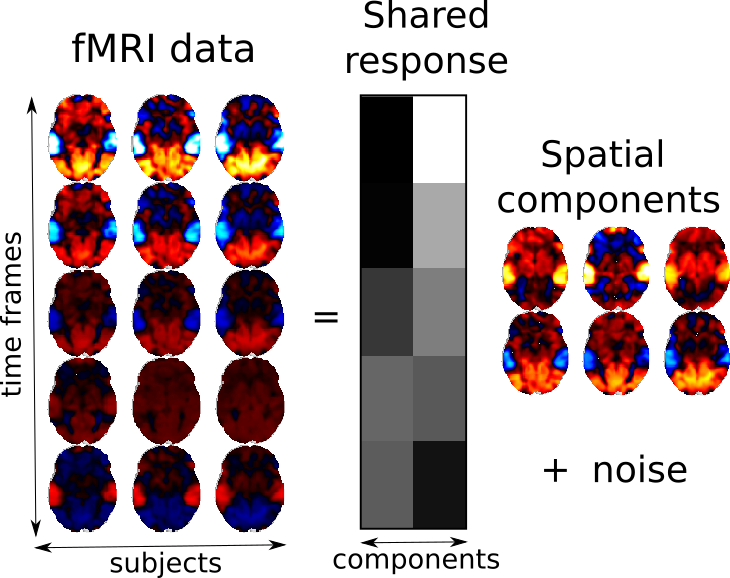
\includegraphics[scale=0.3]{figures/srm/conceptual_figure33.png}
  \caption{\textbf{Shared response model}: The raw fMRI data are modeled as a
    weighted combination of subject-specific spatial components with additive
    noise.
    %
    The weights are shared between subjects and constitute the shared response
    to the stimuli.
    %
  }
  \label{fig:srm:conceptual_figure}
\end{figure}


\subsection{Deterministic shared response model}
\label{sec:deterministicsrm}
Let us consider $n$ observations (scans) of $\xb_i$ and $\sbb$ that we stack into
matrices $X_i \in \RR^{v, n}$ and $S \in \RR^{p, n}$.
%
The deterministic shared response model considers both the mixing matrices $A_i$ and
the $n$ observations of the shared response $S$ as parameters to be
estimated.
%
The noise variance is fixed to a multiple of identity: $\forall i,
\Sigma_i=\sigma^2 I_v$ where $\sigma$ is an hyper-parameter to choose.


The model is optimized by maximizing the log-likelihood, assuming that
the noise is Gaussian distributed.
%
The likelihood is then given by: $p(\xb) = \prod_i \Ncal(\xb_i; A_i \sbb, \sigma^2 I)$ and
therefore the empirical
%
% \textbf{XXX why expected ?} It was for empirical expectation but it may be
% confusing so I removed it.
%
negative log-likelihood is given up to a constant independent of
$A_i$ and $S$ by:
\begin{align}
  \loss = \frac1{n} \sum_i \|A_i S - X_i \|^2 = \frac1{n} \big(\| S \|^2 -2 \dotp{ A_i S}{ X_i } + \| X_i \|^2 \big)
  \label{eq:detsrmloss}
\end{align}
$\loss$ is optimized by performing alternate minimization on $(A_1 \dots A_m)$
and $S$.
%
Note that the hyper-parameter $\sigma$ does not have an influence on
the loss and can therefore be ignored.



The gradient with respect to $S$ is given by $\sum_i A_i^{\top}(A_i S -
X_i) = \sum_i (S - A_i^{\top} X_i)$
yielding the closed form updates:
\begin{equation}
  S \leftarrow  \frac1m \sum_i (A_i^{\top} X_i)
  \label{eq:srm:supdate}
\end{equation}

From \eqref{eq:detsrmloss}, minimizing $\loss$ with respect to $A_i$ is
equivalent to maximizing $\dotp{ A_i}{ X_i S^{\top} }$ and therefore we
have:
\begin{equation}
  A_i \leftarrow  \Pcal \left(\frac1{n}X_i S^{\top} \right)
  \label{eq:detsrm:Aiupdate}
\end{equation}
where $\Pcal$ is the projection on the Stiefel manifold: $\Pcal(M) = M
(M^{\top}M)^{-\frac12}$.
%


The complexity of Deterministic SRM is in $\bigO(\mathrm{n_{iter}} mpvn)$, where
 $\mathrm{n_{iter}}$ is the number of iterations.
%
We monitor the convergence by computing the $\ell_{\infty}$ norm of the
gradient.
%
Note that we can monitor the gradient without any increase in complexity.
%
Indeed, after the updates with respect to each mixing matrix have been
carried out, the gradient with respect to $(W_i)_{i=1}^m$ is zero and therefore
to compute the $\ell_{\infty}$ norm of the gradient we only need the gradient
with respect to $S$: $m S - \sum_i A_i^{\top}\xb_i$ where the right hand side is
used in the updates of $S$.
%
The algorithm is stopped when the
gradient falls below a chosen tolerance.
%


\subsection{Probabilistic SRM}
\label{sec:probabilisticsrm}
In Probabilistic SRM , $\Sigma_i=\sigma_i^2 I_v$ and the shared
components are assumed to be Gaussian $\sbb \sim \Ncal(0, \Sigma_s)$.
%

In~\cite{chen2015reduced} and~\cite{anderson2016enabling}, $\Sigma_s$ is only assumed to be definite positive.
%
As already highlighted in introduction, this causes the model to be
unidentifiable (see~\cite{richard2020modeling} Appendix D for a proof). Enforcing a diagonal $\Sigma_s$ ensures identifiability, provided that the diagonal values are different.
%
So we assume here that $\Sigma_s$ is diagonal (and refer the interested reader
to~\cite{chen2015reduced} and~\cite{anderson2016enabling} for the original formulation of Probabilistic SRM
without the diagonal constraint)
%



The model is optimized via the expectation maximization algorithm.
%
We give all details on the formulation and derivation of update rules in section \ref{details:probsrm}.
%
Denoting $\VV[\sbb | \xb] = (\sum_i \frac1{\sigma_i^2} I +
\Sigma_s^{-1})^{-1}$ and $\EE[\sbb | \xb] = \VV[\sbb | \xb] \sum_i \frac1{\sigma_i^2}
A_i^{\top}\xb_i$, the updates are given by:
\begin{align}
  &\sigma_i^2 \leftarrow \frac1{v} (\EE[\| \xb_i - A_i \EE[\sbb|\xb]\|^2] + \| \diag(\VV[\sbb | \xb]) \|) \\
  % no square here, right ?
  &A_i \leftarrow \Pcal(\EE[\xb_i \EE[\sbb|\xb]^{\top}]) \label{eq:psrm:Aiupdate} \\
  & \Sigma_s \leftarrow \VV[\sbb | \xb] + \EE[\EE[\sbb | \xb] \EE[\sbb | \xb]^{\top}]
\end{align}


The complexity of Probabilistic SRM is $\bigO(\mathrm{n_{iter}} mpvn)$, the same as in
Deterministic SRM.
%
We can monitor the convergence by computing the log-likelihood decrease at each iteration
and stop the algorithm when the magnitude of the decrease is below some
tolerance.
%
The storage requirements of Deterministic or Probabilistic SRM are in
$\bigO(mvn)$ which simply means that the dataset needs to hold in memory.
%


\section{The FastSRM algorithm}

\subsection{Reducing the computational burden by the use of spatial decompositions}

% \textbf{XXX Sorry but we can't call $U$ and atlas: it does not define regions, it has no sign constraints, it is not sparse etc. It is actually closer to a random projection matrix than two an atlas ! So I propose to systematically remove the term atlas, and use spatial decompositions}

SRM algorithms use different sets of parameters $\theta$ to represent the data.
%
In deterministic SRM $\theta = \left((A_i)_{i=1}^m, S \right)$ where $(A_i)_{i=1}^m$ are the
mixing matrices and $S$ is the shared response, while in probabilistic SRM $\theta
= \left( (A_i)_{i=1}^m, \Sigma_s, (\sigma_i)_{i=1}^m \right) $ where $(A_i)_{i=1}^m$ are the
mixing matrices, $(\sigma_i)_{i=1}^m$ the noise levels and $\Sigma_s$ the
components variance.
%


In fMRI, spatial decompositions are often used to reduce the dimensionality of
the data.
%
A classical approach is to apply a deterministic atlas such
as~\cite{bellec2010multi} which is a parcellation of the
brain into $r$ regions.
%
There also exist probabilistic atlases
such as~\cite{dadi_fine-grain_2020} that describes each region as a set of weights across
the full brain. 
%

Deterministic and probabilistic atlases are spatial decompositions that do not
depend on the view at hand. In FastSRM, we consider a set of view-specific
spatial decompositions
$U_i \in \RR^{v \times r}$ such that
$U_i^{\top}U_i = I_r$ where $r$ is the number of components in the spatial decompositions.
%
Data are reduced using $\zb_i = U_i^{\top} \xb_i$ and an SRM algorithm is applied
on data $\zb_i$ yielding parameters $\theta'$.
%
Figure~\ref{fig:srm:conceptual} illustrates this process.
%


Note that the parameters obtained with FastSRM $\theta'$ are different
from the parameters obtained with the corresponding SRM algorithm $\theta$ (the
unmixing matrices in $\theta'$ do not even have the same shape as the unmixing
matrices in $\theta$).
%
However, as we will see in the next section, there exist spatial decompositions such that the
models parametrized by $\theta$ and
$\theta'$ are equivalent.
%


\begin{figure}
  \centering
  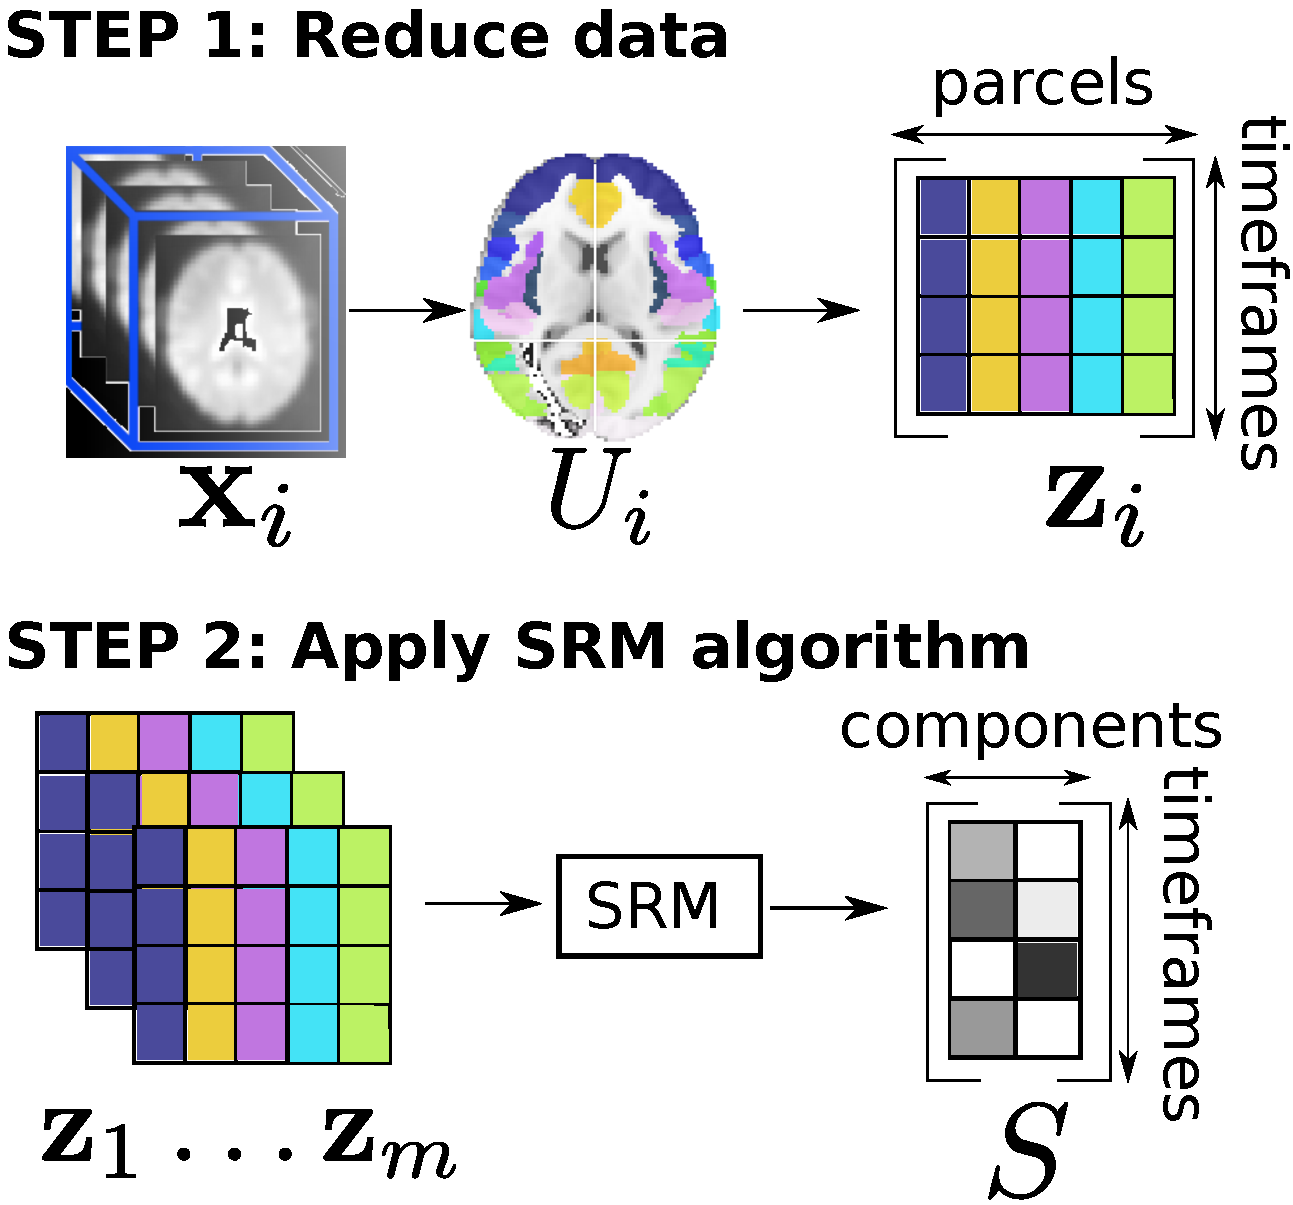
\includegraphics[scale=0.34]{figures/srm/conceptual_figure2.pdf}
  \caption{\textbf{FastSRM algorithm} In step 1, data $\xb_i$ are projected onto a
    spatial decomposition $U_i$ that may depend on the subject $i$ (top).
    %
    In step 2 a SRM algorithm is applied on reduced data to compute the shared
    response.
    %
  }
  \label{fig:srm:conceptual}
\end{figure}

From a computational stand point, dimension reduction provides
a large reduction in memory usage.
%
Indeed as the original data are seen only
once, it is no longer necessary to keep the full dataset in memory (we can load
data $X_i$ one after the other and similarly for the spatial decomposition $U_i$).
%
Therefore
the memory consumption is only in $\bigO(vn)$ (where $v$ is the number of voxels
and $n$ is the number of samples) which is lower than that of SRM by a factor of $m$,
the number of subjects.
%
The number of subjects is typically between $10$ and
$1000$.
%
This yields a practical benefit: on fMRI datasets with many subjects, one no
longer needs a large cluster to run the shared response model but only a modern
laptop.
%
Additionally, low memory consumption reduces the
risk of thrashing~\cite{denning1968thrashing}, a phenomenon that causes large
increase in computation time when the memory used is close to the total available
memory in the hardware.
%


After preprocessing, the reduced representation $\zb_i$ is used instead of the
original data $\xb_i$ yielding a time complexity of $\bigO(
\mathrm{T_{preprocessing}} + \mathrm{n_{iter}} mpnr)$.
%
Let us highlight that an experiment is often run multiple times,
typically when the analysis requires cross-validation procedures.
%
In these cases,
the pre-processing is performed only once and the apparent complexity becomes
$\bigO(\mathrm{n_{iter}} mpnr)$ which is faster than SRM by
a factor of $\frac{v}{r}$.
%
The number of components in large spatial decompositions is about $r=1000$ and in full brain data,
the number of voxels is about $300~000$ so that $\frac{v}{r}$ is typically about
$300$.
%
It remains to be shown how to draw a correspondence between FastSRM
and SRM, which we do in the following section.
%


\subsection{A class of optimal spatial decompositions}
\label{sec:optimal_atlas}
In principle, FastSRM can be used with any spatial decomposition.
%
However, in general, working with reduced data induces a loss of information
that can be minimized if the spatial decomposition is carefully chosen.
%
In any case, there is little hope to recover the parameters that would have been
obtained from SRM from the parameters of FastSRM.
%
Yet, we show that there exists an optimal spatial decomposition in the
sense that SRM and FastSRM yield the same results.


Let us consider $\xb_i = U_{\xb_i} \zb_i$
%
% \bt{But any fill-rank orthogonal basis would work equally well (i.e. any
%   orthogonal transform of the PCA basis)}
%
a PCA of $\xb_i$ with the maximum
number of components.
%
As the number of
samples $n$ is lower than the number of features, $U_{\xb_i} \in \RR^{v \times
  n}$ and $\zb_i \in \RR^{n}$.
%
We also have $U_{\xb_i}^{\top}U_{\xb_i} = I$.
%
Therefore $U_{\xb_i}$ constitutes a possible choice of subject specific spatial decomposition.
%
As the next property shows, $U_{\xb_i}$ is an optimal spatial decomposition for deterministic
FastSRM. Note that this optimal spatial decomposition is not unique: any orthogonal matrix with
the same span as the columns of $X_i$ would also work.
%

\begin{proposition}[Optimal spatial decomposition for deterministic FastSRM]
  Let $(A_i)_i, S$ be the solution obtained by deterministic SRM on data
  $(X_i)_i$ and $(A_i')_i, S'$ the solution obtained by deterministic FastSRM on
  data $(X_i)_i$ using spatial decompositions $(U_{X_i})_i$ where $X_i = U_{\xb_i} Z_i$ is a PCA
  of $X_i$.
  %
  Then $A_i = U_{X_i}A_i'$ and $S = S'$.
  %
  
\label{prop:optimaldetsrm}
\end{proposition}
The proof is available in appendix~\ref{proof:deterministic}.
In the case of probabilistic SRM we can obtain very similar results.
%
However the
algorithm applied on reduced data needs to be slightly modified.
%
We have the following result:
\begin{proposition}[Optimal spatial decomposition for probabilistic FastSRM]
  Let $(A_i)_i, \sigma_i, \Sigma_s$ be the solution obtained by probabilistic SRM on data
  $\xb_i$ and $(A_i')_i, \sigma_i', \Sigma_s'$ the solution obtained by ProbSRM on
  data $\zb_i = U_{\xb_i}^{\top} \xb_i$ but where updates:
  \begin{align}
    \sigma_i^2 \leftarrow \frac1{t} (\EE[\| \zb_i - A_i \EE[\sbb|\zb]\|^2] + \| \diag(\VV[\sbb | \zb]) \|^2)
  \end{align}
  are replaced by updates
  \begin{align}
    \sigma_i^2 \leftarrow \frac1{v} (\EE[\| \zb_i - A_i \EE[\sbb|\zb]\|^2] + \| \diag(\VV[\sbb | \zb]) \|^2)
  \end{align}
  %
  Then $A_i = U_{\xb_i}A_i'$, $\sigma_i =
  \sigma_i'$ and $\Sigma_s = \Sigma_s'$.
  %
  
  \label{prop:optimalprobsrm}
\end{proposition}
  The proof is available in appendix~\ref{proof:prob}.
Proposition~\ref{prop:optimaldetsrm} and Proposition~\ref{prop:optimalprobsrm} show that
no information is lost by replacing $\xb_i \in \RR^v$ by its reduced
representation $\zb_i \in \RR^n$.
%
A key observation is that Proposition~\ref{prop:optimaldetsrm} and
Proposition~\ref{prop:optimalprobsrm} hold whether or
not the model for deterministic (respectively probabilistic) SRM is indeed the
generative model of the data.
%


A complexity analysis shows that finding an optimal spatial decomposition becomes the limiting
step of the pipeline.
%
Even with fast implementations, subject specific PCA
is costly.
%
However FastSRM only works on $\zb_i$ so we do not need to know the value of
$U_{\xb_i}$.
%
In practice, we observe data $X_i \in \RR^{v \times n}$ and we want to get $Z_i
\in \RR^{n \times n}$ such that $X_i = U_{\xb_i} Z_i$.
%
This can be done by performing an
SVD of $X_i^{\top} X_i$ yielding $X_i^{\top}X_i= V_i D_i V_i^{\top}$ and setting
$Z_i = D_i^{\frac12} V_i^{\top}$.
%
Although computing the product $X_i^{\top} X_i$ has time complexity
$\bigO(vt^2)$ (the same as a PCA) the constant in the $\bigO$ is exactly one so
this operation costs a lot less than a PCA
on full data.
%
When estimates of the mixing matrices are needed, they can be obtained by
applying equation~\eqref{eq:fastdetsrm:Aiupdate} in the deterministic SRM case and
equation~\eqref{eq:fastprobsrm:Aiupdate} in the probabilistic SRM case which only costs
$\bigO(mvp^2)$.
%
In practice the cost of the matrix products $X_i^{\top} X_i$ is often the
limiting step of the pipeline (this depends on the number of iterations) but as
we show next, it is much more efficient than performing SRM on
the full data.
%
Note that if large  memory resources are available, these matrix products can be
computed in parallel.
%

\section{Related work}
The implementation of SRM proposed in~\cite{chen2015reduced} is quadratic in the
number of features, which prevents its application to full brain data.
In~\cite{anderson2016enabling}, this issue is addressed by using the
inversion lemma to remove the quadratic dependence. Their implementation is now the most widely used one.
In our work, we propose to reduce further the computation time and memory usage
compared to the implementation in~\cite{anderson2016enabling} by the use of
optimal spatial decompositions.

Other popular methods used to speed up SRM are searchlight~\cite{zhang2016searchlight} or piecewise~\cite{bazeille2021empirical}
approaches. While these methods are efficient, they do not optimize the same
objective as the original SRM algorithm and are arguably less principled since the
searchlights or pieces are chosen a priori.

We consider SRM as a well principled formulation of the hyperalignment
method~\cite{haxby2011common}.
%
Many methods exist to perform hyperalignment: deep
hyperalignment~\cite{yousefnezhad2017deep} , robust
SRM~\cite{turek2018capturing} , multi-view canonical correlation
analysis~\cite{li2009joint}, ShICA~\cite{richard2021model},
MultiViewICA~\cite{richard2020modeling} optimal
transport~\cite{bazeille2019local} and many more.
%
In this work, we do not discuss the merit of FastSRM with respect to
other methods. We simply observe that SRM is widely used and aim to provide
a faster, more memory efficient and identifiable implementation.  In
our view, FastSRM should be used as a plugin replacement for SRM.


\section{Experiments}
We make several experiments on both synthetic and real data.
%
We used Nilearn~\cite{abraham2014machine} (version 0.8.1) for fMRI data preprocessing,
Brainiak~\cite{kumar2020brainiak2} (version 0.9) for the non-identifiable version of SRM that
implements the work of~\cite{chen2015reduced} and~\cite{anderson2016enabling},
Numpy~\cite{harris2020array} (version 1.19.0) for
array processing, Scipy~\cite{2020SciPy-NMeth} (version 1.5.3) its implementation of the
Hungarian algorithm, Matplotlib~\cite{hunter2007matplotlib} (version 3.1.2) for plotting and
Sklearn~\cite{pedregosa2011scikit} (version 0.23.2) for machine learning pipelines.

\subsection{Comparing Fitting time and performance of FastSRM and
  SRM on synthetic data}
We generate synthetic data $\xb_i$ according to the model of probabilistic SRM.
%
The parameters $\sigma_i^2$, $A_i$ and $\Sigma_s$ are generated randomly.
%
We sample the value of the subject specific noise level from a normal
distribution: $\sigma_i \sim \Ncal(0, 0.1)$
%\bt{$\sigma_i$ has to be non-negative}.
% No only $\sigma_i^2$.
%
The mixing matrices $A_i$
are obtained by sampling their coefficient from a standardized normal
distribution.
%
Lastly, the covariance of the shared response $\Sigma_s$ is diagonal and the
diagonal values are obtained by sampling from a Dirichlet distribution with
parameter $(1 \dots 1)$.
%
We set the number of voxels to $v=125~000$, the number of subjects to $m=10$ and
the number of components to $p=50$.
%
We generate $n=1000$ samples.
%


We benchmark deterministic SRM, probabilistic SRM and their FastSRM counterparts in terms of fitting time and performance.
%
Note that in this section, the identifiable implementation of deterministic SRM
and probabilistic SRM described in section~\ref{sec:probabilisticsrm}
and~\ref{sec:deterministicsrm} is used. 
%
Algorithms are designated by the spatial decomposition they use and therefore SRM algorithms are referred to
as \emph{None} because no spatial decomposition is used and FastSRM algorithms will have the
label \emph{Optimal}.
%
Note that it would be possible to use FastSRM with sub-optimal
spatial decompositions (there exists a wide variety of brain spatial decompositions
~\cite{schaefer2017local, bellec2010multi, mensch2018extracting}) but
using them does not bring any guarantee that the performance is the same as SRM.
%


We use a number of iterations between 1 and 100 and report the performance,
fitting time and a measure of convergence.
%
In FastSRM, we do not compute the
unmixing matrices but only the shared response.
%
We measure the performance of an algorithm by computing the error between the true component $S \in \RR^{p \times n}$ and
the predicted component $\hat{S} \in \RR^{p \times n}$ using the quantity:
\begin{align}
\mathrm{mse}(\hat{S}, S) = min_{B \in \RR^{p \times p}} \|B \hat{S} - S \|^2_F =  \|S
\hat{S}^{\dagger}\hat{S} - S \|^2_F
\end{align}
%
This way of measuring errors is
insensitive to the indeterminacies in DetSRM.
%
We measure the fitting time in seconds.
%
Lastly, we measure convergence by computing the gradient $\ell_{\infty}$ norm in
case of DetSRM given by $\max(\mathrm{abs}(G))$ where $G$ is the gradient and
use the distance between consecutive values of the loss for ProbSRM.
%
Results are plotted in Figure~\ref{fig:srm:synthetic_gradient}.
%

We empirically see that the optimal approach is equivalent to using no spatial decompositions in
terms of performance.
%
This is predicted by the theory in section~\ref{sec:optimal_atlas},
where we demonstrate that these two algorithms yield exactly the same
output from a given input and initialization.
%
% %
% Among approximate methods, the projection
% method yields the best results but are quite far away from optimal results.
%
% %
In general probabilistic methods give much better results than their deterministic
counterpart.
%
This shows the superiority of likelihood based methods.
%
In terms of fitting time, FastSRM is about a thousand time faster than SRM after
100 iterations.
%
When no spatial decomposition is used, the number
of iterations has a very strong impact on performance while it has a small impact
when an optimal spatial decomposition is used.
%
Lastly, looking at the convergence curves, we see that even after $100$ iterations, algorithms did
not fully converge.
%
This means that in practice a larger number of
iterations is needed, which would yield an even higher difference in fitting time
between methods using no spatial decomposition and methods using an optimal
spatial decomposition.
%


\begin{figure}
  \centering
  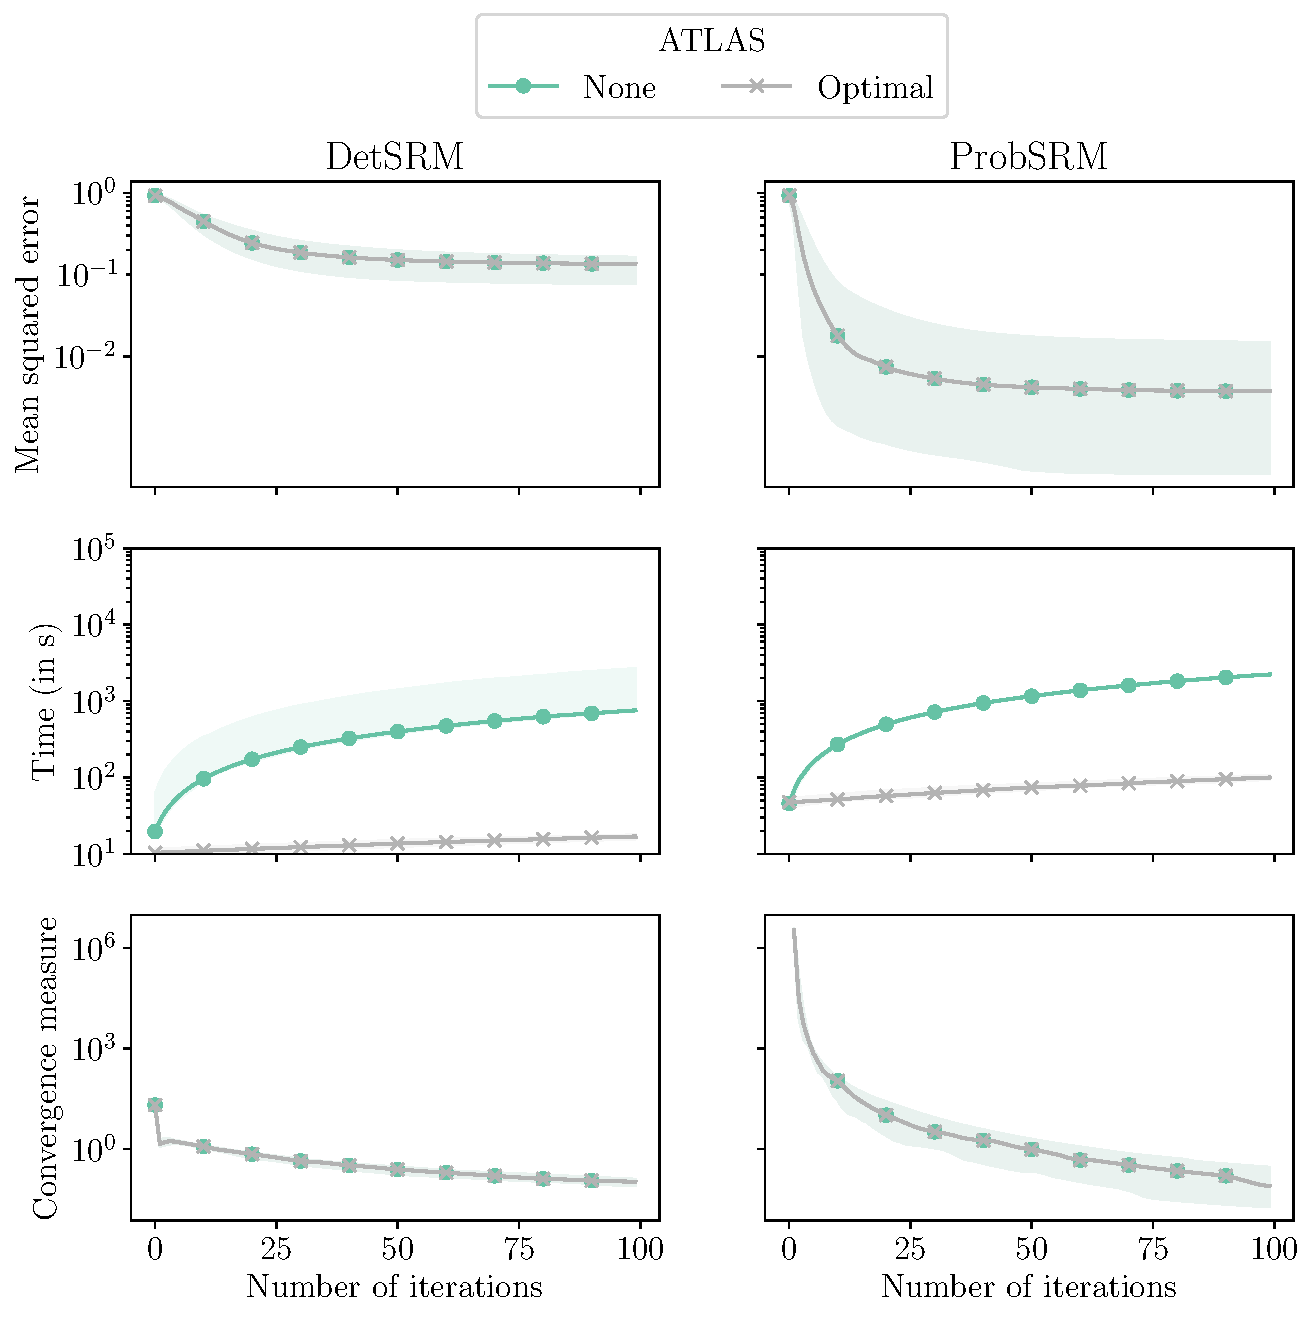
\includegraphics[width=\textwidth]{../figures/synthetic_gradient.pdf}
  \caption{\textbf{Benchmark of SRM algorithms on synthetic data: } Performance,
    fitting time and convergence of SRM algorithms in the deterministic (left)
    or probabilistic (right) case.
    %
    As expected, when optimal spatial decompositions are used,
    the performance is the same as if no spatial decomposition is used but the fitting time is
    much lower.
    %
    This is even more pronounced when the number of iterations is
    high (and looking at convergence curves, we see that more iterations could
    be performed to be closer to a stationary point).
    %
  }
  \label{fig:srm:synthetic_gradient}
\end{figure}

\subsection{Experiment on fMRI data: identifiability increases stability}
We evaluate the performance of the different SRM implementations on the
\emph{Sherlock} datasets where fMRI of 17 participants watching "Sherlock" BBC
TV show (episode 1) is performed.
%
% 
These data are downloaded from
\url{http://arks.princeton.edu/ark:/88435/dsp01nz8062179}.
%
% 
Data were acquired using a 3T scanner with an isotropic spatial resolution of
3~mm.
%
% 
More information including the preprocessing pipeline is available in
\cite{sherlock}.
%
% 
Subject 5 is removed because of missing data, leaving us with 16 participants.
%
Although SHERLOCK data originally contain 1 run only, we split them into 4 blocks
of 395 time frames and one block of 396 time frames for the needs of our
experiments.
%



We first show that identifiability is a desirable property as it increases
stability.
%
Then we show that our FastSRM algorithm (that works with optimal spatial decompositions)
matches the performance of SRM (that works on full data) but use much less
computational resources.
%


\subsection{Identifiability increases stability}
Assuming that the data follow the model, identifiability ensures that the
problem is well-posed since the solutions are well-characterized. Note however that SRM
remains non-convex so there is no guarantee that the optimal solution is found.
%
% \bt{I find this a bit ambiguous: you give te impression that you gurantee that the optimal solution is used. Rephrase.}
%
In real fMRI data, the model cannot be expected to hold perfectly, but we can
hope for greater stability in the parameters recovered than if an non-identifiable
model is used.


To measure the stability of the shared components obtained from the Sherlock
dataset, we divide the subjects into two roughly equal groups and extract the
common components in each group.
%
The components are then matched using the Hungarian algorithm and the stability
measure is obtained from the average correlation of the matched components.
%
The procedure is repeated 9 times using the Brainiak implementation (that is not
identifiable since the shared components covariance is unconstrained) and our
FastSRM implementation.
%
We plot the results as a scatter plot in
Figure~\ref{exp:identifiability}, where, for each repetition, the
x-axis indicates the stability measure obtained with Brainiak's
implementation and the y-axis the stability measure obtained with
FastSRM (identifiable since the shared components covariance is
diagonal).
%
We see that introducing a diagonal source covariance improves stability.
%


\begin{figure}
\begin{minipage}{0.38\linewidth}
      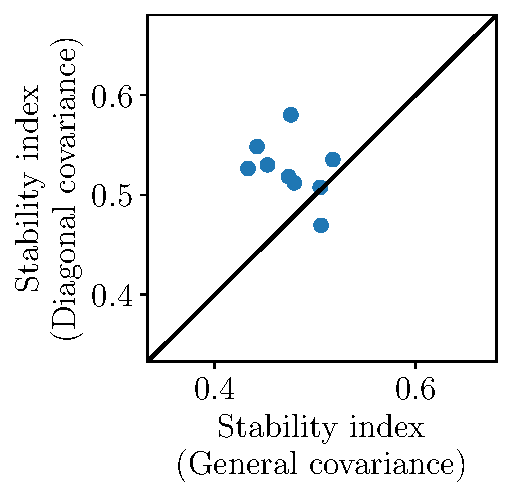
\includegraphics[width=\textwidth]{../figures/identifiability.pdf}
    \end{minipage}
    \hfill
    \begin{minipage}{0.6\linewidth}
        \caption{\label{exp:identifiability}\textbf{Identifiability increases
            stability: } We first divide the subjects
          into two groups and extract the common components in each group.
          %
          The components of the two groups are then matched using the Hungarian
          algorithm and the stability index is determined by the average
          correlation of the matched components.
          %
          The procedure is repeated 9 times with the Brainiak implementation
          (not identifiable since the shared components covariance is unconstrained) and our FastSRM implementation
          (identifiable since the shared components covariance is diagonal).
          %
        }
    \end{minipage}
\end{figure}


\subsection{Comparing fitting time, memory usage and performance on a
  timesegment matching experiment}
\label{sec:timesegment_expe}
\label{timesegment_expe}
Time-segment matching has first been introduced
in~\cite{chen2015reduced}.
%
In a nutshell, the time-segment matching accuracy measures the similarity
between two multivariate time-series by trying to localize a time-segment in one
time-series by correlation with the other.
%
In the context of movie watching, this measure is quite meaningful: if
we split the movies in scenes and compute a representation per scene
and per subject, it can be assumed that different subjects watching
the movie would still have closer representation of the same scenes
than of different scenes.
%
This explains why timesegment matching is a standard evaluation of SRM-like methods also used in  \cite{guntupalli2018computational}, \cite{Nastase741975} or
\cite{zhang2016searchlight}.
%


We now describe more precisely the experimental design.
%
We split the runs into a train and test set.
%
After fitting the model on the
training set, we apply the unmixing matrices $W_i=A_i^{-1}$ of each subject on
the test set yielding individual components matrices.
%
We estimate the shared responses by averaging the individual components of each
subject but one.
%
We select a target time-segment (9 consecutive time frames) in the shared
responses and try to localize the corresponding time segment in the components
of the left-out subject using a maximum-correlation classifier.
%

The time-segment is said to be
correctly classified if the correlation between the sample and target
time-segment is higher than with any other time-segment (partially overlapping
time windows are excluded).
%

% 
We use 5-Fold cross-validation across runs: the training set contains 80\% of
the runs and the test set 20\%, and repeat the experiment using all possible
choices for left-out subjects.
%
% 
The mean accuracy is reported in Figure~\ref{fig:srm:timesegment} (top).
%
When an optimal spatial decomposition is used, the accuracy is the same as when no
spatial decomposition is used but the fitting time is reduced by a factor 10 to 100
and so is the memory usage (see Figure~\ref{fig:srm:timesegment},
bottom).
%

% 

\begin{figure}
  \centering
  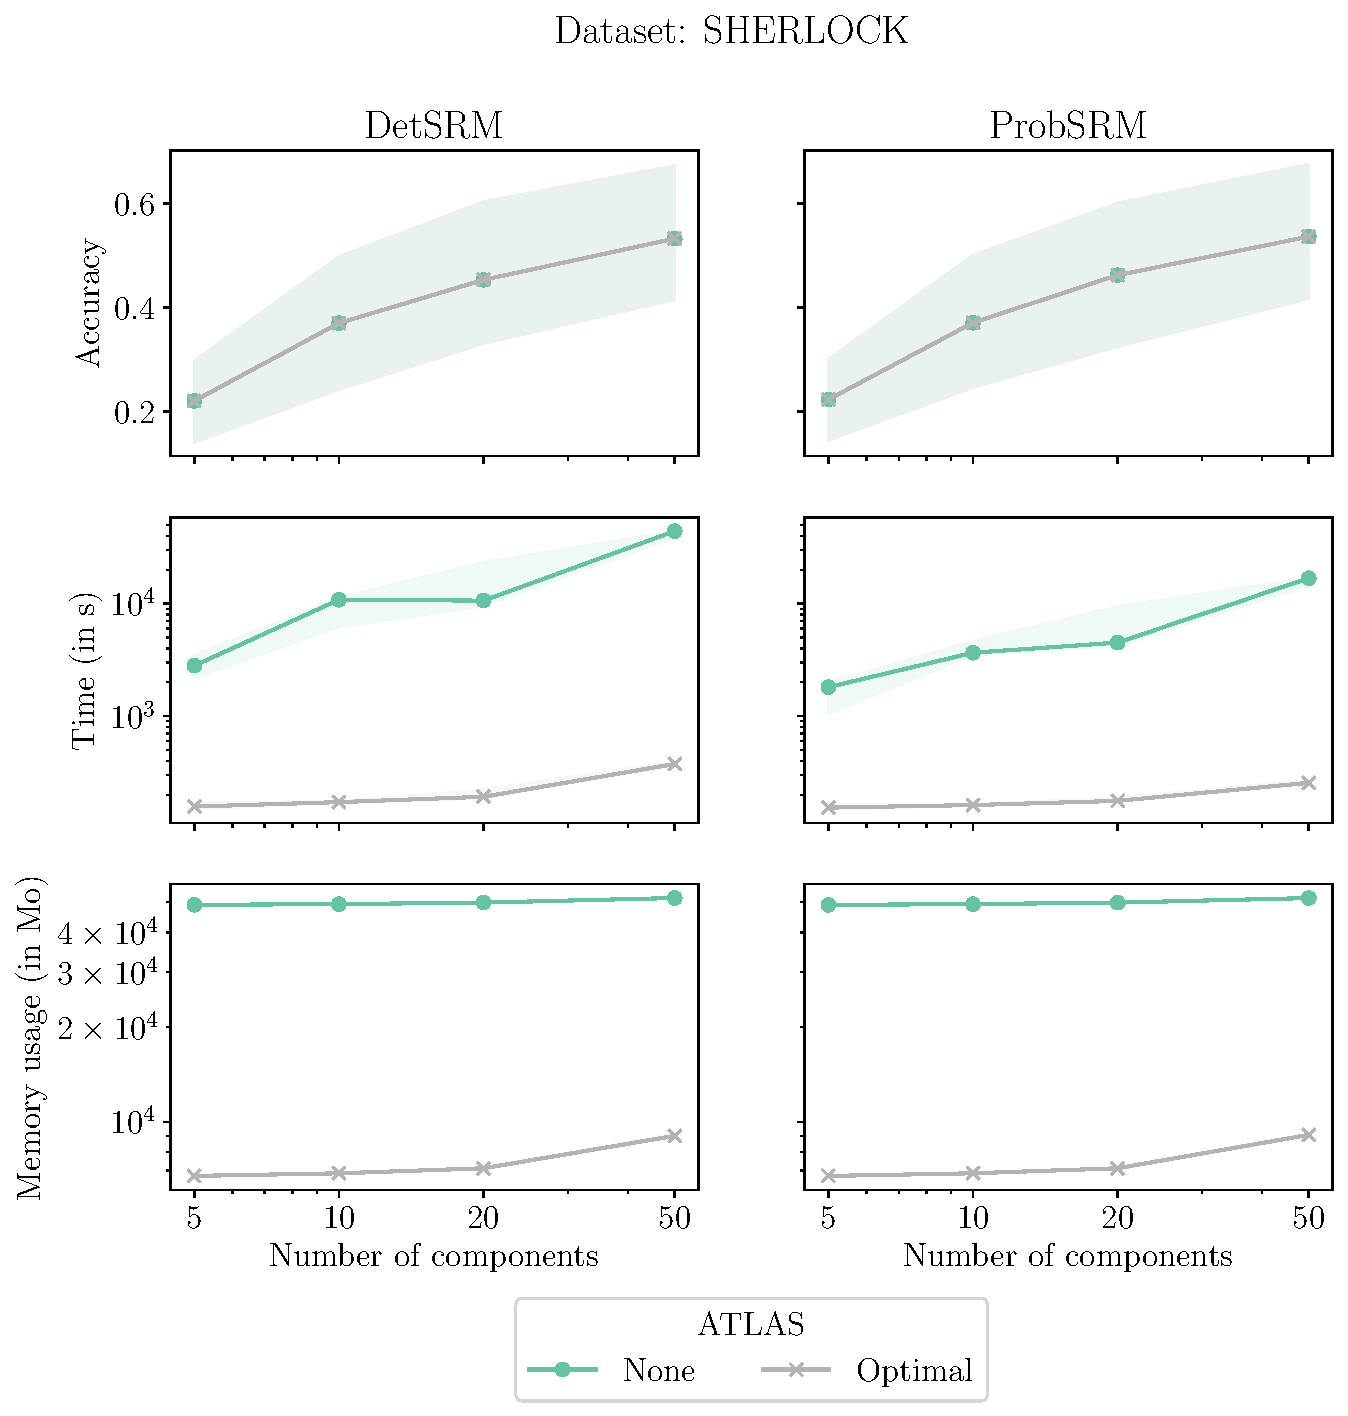
\includegraphics[width=0.8\textwidth]{../figures/timesegment_matching_sherlock.pdf}
  \caption{\textbf{Benchmark of SRM algorithms on fMRI data} (top) Timesegment
    matching accuracy (middle) Fitting time (bottom) Memory usage. When the
    optimal spatial decomposition is used, the accuracy is the same as when no
    spatial decomposition is used but
    the fitting time is reduced by a factor 10 to 100 and so is the memory usage.
    %
  }
  \label{fig:srm:timesegment}
\end{figure}

\section{Implementation and reproducibility}
Our work is fully reproducible and our code is tested and well documented. All
material is available in our github repository \url{https://github.com/hugorichard/FastSRM}.

The API is reminiscent of the scikit-learn one where the model object is
instantiated with its parameters and then fitted on data via a method
\emph{fit()}. After the model is fit, the learned parameters can be accessed.
Then, a \emph{transform()} method computes the shared
response from the learned parameters and the data passed as the argument of the \emph{transform()} method.

While brainiak and nilearn are useful to reproduce some of our experiments, they
are not strong dependencies and FastSRM only needs Numpy ($\geq 1.12$), Scipy
($\geq 0.18.0$), Matplotlib ($\geq 2.0.0$), Scikit-learn ($\geq 0.23$), Pytest
($\geq 6.2.5$) , and Joblib ($\geq 1.1.0$).

The package comes with a documentation and a tutorial that reproduces, at a
smaller scale, the experiment available in Figure~\ref{fig:srm:synthetic_gradient}.
These are found at \url{https://hugorichard.github.io/FastSRM/index.html}.
The instructions to fully reproduce the experiments presented in the papers are
available in the README:
\url{https://github.com/hugorichard/FastSRM/blob/master/README.md}.

A set of tests reduces the risk of introducing a bug. These tests are run any
time a pull request or a merged is performed on the main codebase.

\section{Conclusion}
As studies using naturalistic stimuli will tend to become more common
within and across subjects, we need scalable models in terms of computation time
and memory usage.
%
This is particularly related to the development of deep phenotyping
models such as the Courtois project on Neural Modeling (see \url{https://docs.cneuromod.ca}).
%
This is precisely what FastSRM provides.

FastSRM is an efficient implementation of SRM
that uses optimal spatial decompositions to speed up computations and reduce memory requirements
with provably no loss of performance. 
Note that the new memory requirements do not depend on the number of subjects.
This is really interesting as it would make it possible to apply FastSRM on
datasets with a very large number of subjects that do not hold in memory.

We show on synthetic and real data that FastSRM is much faster and more memory
efficient that implementations not using an optimal spatial decomposition.
Furthermore, FastSRM is identifiable. On real data, we show that compared to
Brainiak's implementation, that is not identifiable, FastSRM provides more
stable estimates of the shared components.

FastSRM inherits from all the weaknesses of SRM including the fact that
mixing matrices are assumed to be orthogonal, which is debattable in practice.
%
It is an open question whether dimension reduction and learning of the shared
components could be done jointly and efficiently without assuming orthogonal
mixing matrices.
%
Our approach based on optimal spatial decomposition shows that SRM-like methods do not need the
full data to provide accurate estimates of shared components. We believe that such
insights may guide the design of future methods.

Last, FastSRM is useful when the number of features is much larger than the
number of samples. This setting is common in fMRI but less common in MEG/EEG where
the number of samples is usually much larger than the number of features. Even
in this case, it is possible to considerably speed up SRM. Indeed, SRM only
depends on second order statistics.
These statistics can be pre-computed making the rest of the
pipeline insensitive to the number of samples in the dataset. An implementation
of this simple idea would make SRM easily applicable to other modalities.
We leave it to future work.
% \bt{Add a paragraph on implementation, sofwtare quality, documentation, examples, availability...}
% \bt{Discuss the use for other brain imaging modelities (MEEG) if relevant ?}

\bibliographystyle{plain}
\bibliography{utils/biblio}


\newpage
\appendix

\section{Detailed derivation of the Probabilistic SRM algorithm}
\label{details:probsrm}
Here we describe in detail the log-likeihood underlying the
Probabilistic SRM and derive the update rules.
%
Denoting $\VV[\sbb | \xb] = (\sum_i \frac1{\sigma_i^2} I +
\Sigma_s^{-1})^{-1}$ and $\EE[\sbb | \xb] = \VV[\sbb | \xb] \sum_i \frac1{\sigma_i^2}
A_i^{\top}\xb_i$, we have

\begin{align}
  p(\xb, \sbb) &= \prod_i \frac{\exp \left(-\frac{\|\xb_i - A_i \sbb \|^2}{2 \sigma_i^2} \right) }{(2 \pi \sigma_i^{2v})^{\frac12}} \frac{\exp(-\frac12 \dotp{ \sbb }{ \Sigma_s^{-1} \sbb } )}{(2 \pi | \Sigma_s|)^{\frac12}} \\
               &= c_1 \exp (-\frac12 \left( \sum_i \frac1{\sigma_i^2}\|\xb_i\|^2 - 2  \dotp{ \sum_i \frac1{\sigma_i^2} A_i^{\top}\xb_i}{ \sbb } \right. \\& \left.+ \sum_i \frac1{\sigma_i^2} \| \sbb \|^2 + \dotp{ \sbb}{ \Sigma_s^{-1} \sbb }  \right)) \\
               &= c_2(\xb) \exp(-\frac12 \left( \dotp{  \sbb - \EE[\sbb }{ \xb], \VV[\sbb | \xb]^{-1} ( \sbb - \EE[\sbb | \xb])  } \right)) \label{probsrmcompleted}
\end{align}
where
\begin{align}
  c_1 = \frac1{(2 \pi \sigma_i^{2v})^{\frac12}}\frac1{(2 \pi |
  \Sigma_s|)^{\frac12}}
\end{align}
and
\begin{align}
  c_2(\xb) = c_1 \exp \left( -\frac12 \left( \sum_i \frac1{\sigma_i^2}\|\xb_i\|^2 - \dotp{  \EE[\sbb }{ \xb], \VV[\sbb | \xb]^{-1} \EE[\sbb | \xb] } \right) \right)
\end{align}
are independent from $\sbb$.
%
Therefore,
\begin{align}
  \sbb| \xb \sim \Ncal(\EE[\sbb | \xb], \VV[\sbb, \xb])
\end{align}

The negative expected completed log-likelihood is given by
\begin{align}
	\loss = \sum_i \frac12 v \log(\sigma_i^2) + \frac1{2 \sigma_i^2} \EE[\| \xb_i - A_i \sbb \|^2]
\end{align}
updates are therefore given by:
\begin{align}
  &\sigma_i^2 \leftarrow \frac1{v} (\EE[\| \xb_i - A_i \EE[\sbb|\xb]\|^2] + \| \diag(\VV[\sbb | \xb]) \|) \\
  % no square here, right ?
  &A_i \leftarrow \Pcal(\EE[\xb_i \EE[\sbb|\xb]^{\top}]) \label{eq:psrm:Aiupdate} \\
  & \Sigma_s \leftarrow \VV[\sbb | \xb] + \EE[\EE[\sbb | \xb] \EE[\sbb | \xb]^{\top}]
\end{align}

It is useful to access the log-likelihood to check the implementation of the
algorithm and monitor the convergence.
%
From equation~\eqref{probsrmcompleted},
the likelihood is given by:
\begin{align}
  p(\xb) &= c_2(\xb) \int_{\sbb} \exp(-\frac12 \left( \dotp{  \sbb - \EE[\sbb }{ \xb], \VV[\sbb | \xb]^{-1} ( \sbb - \EE[\sbb | \xb])  } \right)) d\sbb \\
         &= c_2(\xb) (2 \pi |\VV[\sbb | \xb]|)^{\frac12}
\end{align}
replacing $c_2(\xb)$ by its expression and taking the log, the expected negative
log-likelihood is (up to constants) given by:
\begin{align}
  \EE[-\log(&p(\xb))] = \sum_i \frac{v}{2} \log(\sigma_i^2) + \frac12 \log(|\Sigma_s|) - \frac12 \log(|\VV[\sbb | \xb]|) \nonumber \\ &+ \sum_i
  \frac12 \frac1{\sigma_i^2} \EE[\|\xb_i\|^2] - \frac12 \EE[\dotp{  \EE[\sbb }{ \xb], \VV[\sbb | \xb]^{-1} \EE[\sbb | \xb] }]
\end{align}


\section{Proofs of Proposition~\ref{prop:optimaldetsrm}}
\label{proof:deterministic}

\begin{proof}
Updates of the mixing matrices $A_i$ in deterministic SRM
equation~\eqref{eq:detsrm:Aiupdate} can be written:
\begin{align}
  A_i &\leftarrow \Pcal \left(\frac1{n}X_i S^{\top} \right)= U_{X_i}\Pcal \left(\frac1{n}Z_i S^{\top} \right)
  \label{eq:fastdetsrm:Aiupdate}
\end{align}
where $\Pcal$ is the projection on the Stiefel manifold: $\Pcal(M) = M
(M^{\top}M)^{-\frac12}$.
%

Therefore we can look for $A_i$ as $A_i = U_{X_i} \tilde{A}_i$.
%
We can show that $\tilde{A}_i$ is orthogonal.
%
Indeed,
\begin{align}
  &A_i^{\top} A_i = I_p \\
  & \implies \tilde{A}_i^{\top}U_{X_i}^{\top} U_{X_i} \tilde{A}_i = I_p \\
  & \implies \tilde{A}_i^{\top} \tilde{A}_i = I_p
\end{align}

Then, we use the fact that
\begin{align}
  \|X_i - A_i S \|^2 = \| U_{X_i}Z_i - U_{X_i}\tilde{A}_i S\|^2 = \| Z_i - \tilde{A}_i S \|^2
  \label{eq:equality:xy}
\end{align}
so that $A_i' = \tilde{A}_i$.
%


Therefore, the solution of deterministic SRM on data $(\zb_i)_{i=1}^m$ and
$(\xb_i)_{i=1}^m$ are linked by the change of parameters $A_i = U_{\xb_i}A_i'$ and
$S = S'$.
%
This concludes the proof.
%

\end{proof}


\section{Proofs of Proposition~\ref{prop:optimalprobsrm}}
\label{proof:prob}
\begin{proof}
  Updates of the mixing matrices $A_i$ in probabilistic SRM
  equation~\eqref{eq:psrm:Aiupdate} can be written:
  \begin{align}
    A_i &\leftarrow U_{\xb_i}\Pcal(\EE[\zb_i \EE[\sbb| \xb_i]^T])
    \label{eq:fastprobsrm:Aiupdate}
  \end{align}
  so we can look for $A_i$ as $A_i = U_{\xb_i} \tilde{A}_i$ and, as in the
  deterministic case, $\tilde{A}_i$ is orthogonal.
  %
  Therefore equality~\eqref{eq:equality:xy} holds.
  %
  
  
  Then we consider the expected negative log-likelihood of probabilistic srm:
  \begin{align}
    \loss &= \sum_i \frac12 v\log(\sigma_i^2) + \frac12 \log(|\Sigma_s|) + \EE[\int_{\sbb} \sum_i \frac1{2 \sigma_i^{2}} \|\xb_i - A_i \sbb \|^2 \nonumber \\& \enspace \enspace \enspace \enspace+ \frac12 \dotp{ \sbb }{ \Sigma_s^{-1} \sbb }  d\sbb] \\
          &= \sum_i \frac12 v \log(\sigma_i^2) + \frac12 \log(|\Sigma_s|) + \EE[\int_{\sbb} \sum_i \frac1{2 \sigma_i^{2}}\|\zb_i - \tilde{A}_i \sbb \|^2 \nonumber \\& \enspace \enspace \enspace \enspace+ \frac12 \dotp{ \sbb }{ \Sigma_s^{-1} \sbb }  d\sbb]
  \end{align}
  where we use equality~\eqref{eq:equality:xy}.
  %
  %
  Optimizing the log-likelihood via expectation maximization yields the exact
  same updates as probabilistic SRM on data $\zb_i$
  except that updates
  \begin{align}
    \sigma_i^2 \leftarrow \frac1{t} (\EE[\| \zb_i - \tilde{A}_i \EE[\sbb|\zb]\|^2] + \| \diag(\VV[\sbb | \zb]) \|^2)
  \end{align}
  are replaced by updates
  \begin{align}
    \sigma_i^2 \leftarrow \frac1{v} (\EE[\| \zb_i - \tilde{A}_i \EE[\sbb|\zb]\|^2] + \| \diag(\VV[\sbb | \zb]) \|^2)
  \end{align}
  so that $\tilde{A}_i = A'_i$.
  %
  Therefore, the updates in both algorithms are linked  by $A_i = U_{\xb_i}A_i'$,
  $\sigma_i' =
  \sigma_i$ and $\Sigma_s'  = \Sigma_s$.
  %
  This concludes the proof.
  %
\end{proof}
\end{document}
